\section{Corrientes marinas}

Una de las corrientes marinas que más impacto puede tener en nuestro baño en el mar, es la corriente de resaca. \cite{RESACA}
Una corriente de resaca o corriente de retorno es una fuerte corriente superficial (o casi superficial) de agua, que retrocede desde la costa hacia el mar. Se genera principalmente por el rompimiento irregular de las olas a lo largo de la cresta, llegando bruscamente a la playa con un índice elevado de energía, desvaneciéndose luego sobre el fondo para, posteriormente, regresar hacia el mar por un canal a través de las olas.

Su intensidad depende de la altura de las olas y de las características topográficas de la orilla, siendo además reforzadas por las corrientes de marea, por lo que se hacen más peligrosas en bajamar. Estas corrientes pueden ser visibles o no dependiendo de la intensidad de la corriente y del tipo de sedimento que se encuentra en la playa.

\begin{figure}[hb]
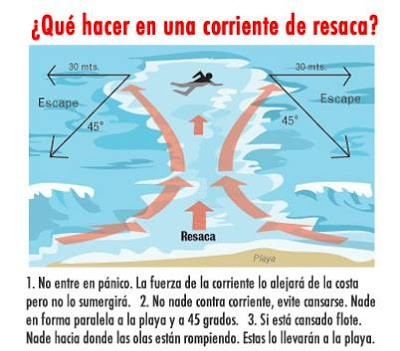
\includegraphics[scale=1.05]{corriente_resaca.jpg} 
\floatfoot{Figura 1. Corriente de resaca}
\end{figure}

Aunque puede no ser un factor de riesgo en deportes acuaticos de vela como el windsurf o kitesurf, es un elemento a tener en cuenta en otras modalidades sin vela como el surf o el paddle surf. Sobretodo si estamos cansados después de una sesión de dos horas o más de deporte, es posible que no podamos salir de las corrientes con facilidad incluso quedar a la deriva por una lipotimia. Este es un caso en el que nuestra aplicación puede tener una utilidad real.
